\begin{figure}[!h]
  \centering
  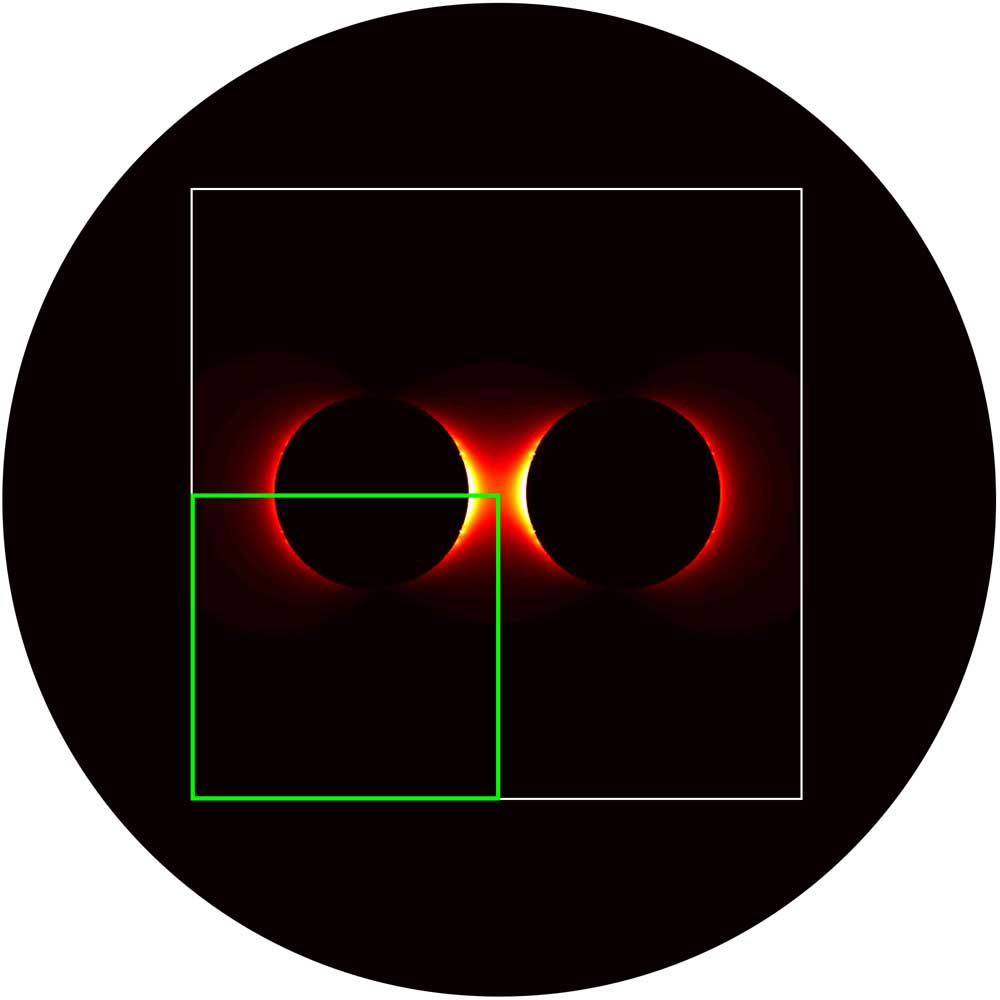
\includegraphics[width=0.5\textwidth]{./images/fwhm-chart.jpg}
  \label{symmetry}
  \caption{The simulated square area (green box) compared to the calculated area (white box) compared to the total area measured by the laser (approximated as circle). The laser has a fwhm of \SI{570}{nm} according to \cite{heeg}.}
\end{figure}

\note{average of slice, compare to total size of laser spot}

\newpage
\null
\newpage
